\documentclass[]{article}

\usepackage[utf8]{inputenc}
\usepackage{amsmath}
\usepackage{amssymb}
\usepackage{amsthm}
\usepackage{amsfonts}
\usepackage{graphicx}
\usepackage{capt-of}
\usepackage{listings}
\usepackage{siunitx}
\usepackage[section]{placeins}
\usepackage{float}



% Oppgavenummerering %
\renewcommand\thesection{Task \arabic{section}}
\renewcommand\thesubsection{\alph{subsection})}

% Bevis
\newcommand\TombStone{\rule{.5em}{.5em}}
\renewcommand\qedsymbol{\TombStone}
\renewcommand{\proofname}{Bevis.} % Norske bevis

\DeclareMathOperator{\Var}{\text{Var}}
\DeclareMathOperator{\Cov}{\text{Cov}}
\DeclareMathOperator{\E}{\text{E}}

\title{Assignment 2}
\author{Sigurd Totland | MTTK}

\begin{document}
\maketitle

\section{}
\subsection{}
We define the events $R_k$, $S_k$, and $E_k$ to denote that the boat is in the area, stays in the area and enters the area, respectively. We then obtain
\begin{equation}\begin{aligned}
r_{k+1|k} &= \Pr(R_{k+1}) \\
&= \Pr(R_k \cap S_k) + \Pr(\neg R_k \cap E_k) \\
&= \Pr(R_k) P_S + \Pr(\neg R_k) P_E \\
&= r_k P_S + (1-r_k) P_E.
\end{aligned}\end{equation}

\subsection{}
The a posteriori probability for the boat being in the region is calculated in the same fashion. We let $D$ denote the event in which the boat is detected, hence obtaining
\begin{equation}\begin{aligned}
r_{k+1} = \Pr(D) = r_{k+1|k} P_D + (1-r_{k+1|k})P_{FA}.
\end{aligned}\end{equation}
The bayesian tree for this task is shown in figure \ref{fig:bayes_tree}.
\begin{figure}[H]
\centering
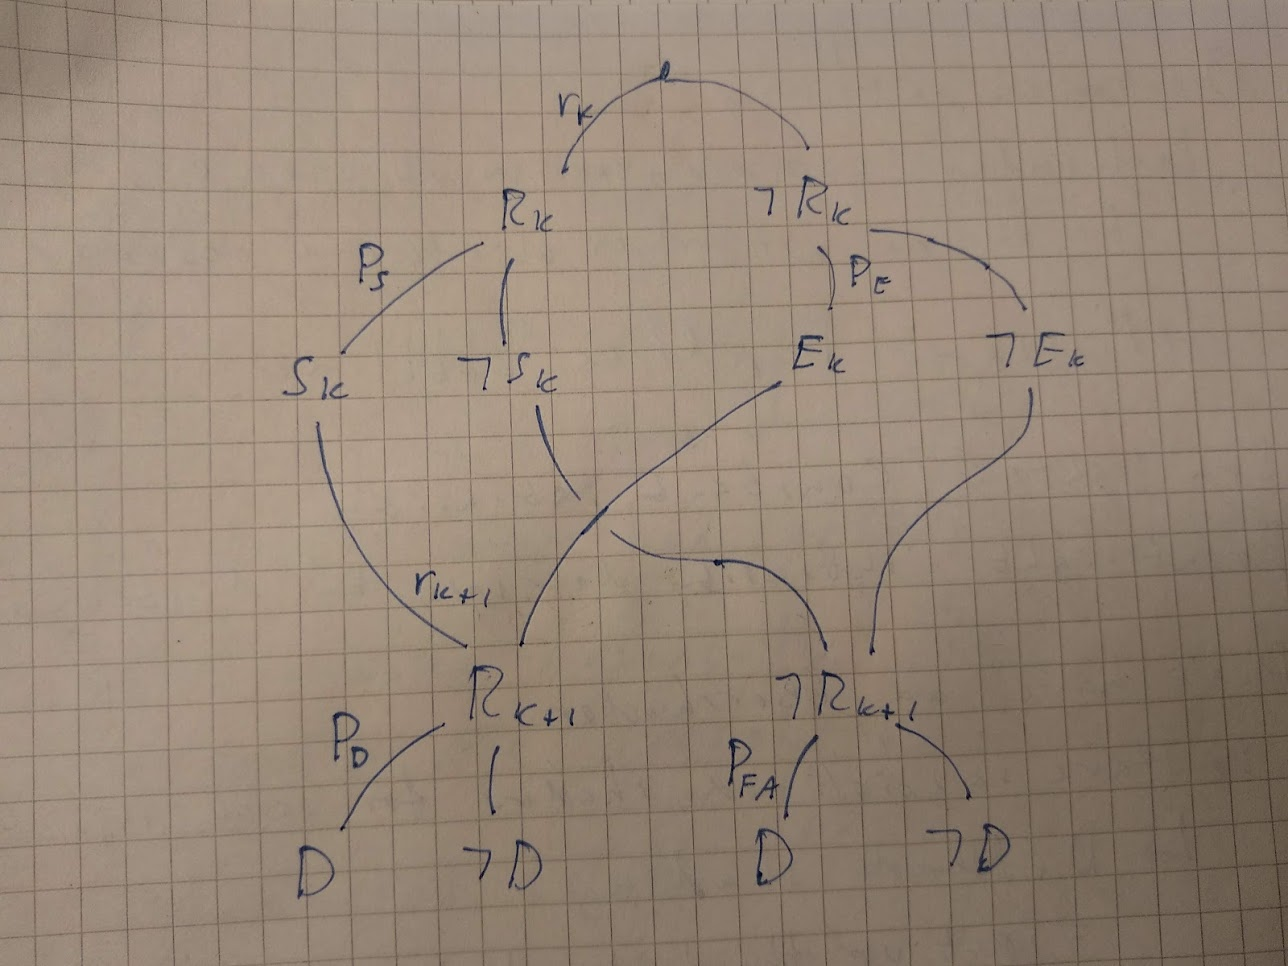
\includegraphics[width=0.6\columnwidth]{bayes.jpg}
\caption{Bayesian tree for boat detection.}
\label{fig:bayes_tree}
\end{figure}

\section{}
\subsection{}
We wish to express $z_1$ and $z_0$ with just the states at $k=1$ and the noise. We get
\begin{equation}\begin{aligned}
z_1 &= p_1 + w_1, \quad \text{and} \\
z_0 &= p_0 + w_0
\end{aligned}\end{equation}
since $z_0$ is dependent on $p_0$ we must try and express this in terms of the $k=1$ state. The CV model is given as
\begin{equation}\begin{aligned}
\dot x = Ax + Bu + Gn
\end{aligned}\end{equation}
where $n$ is the process noise and we let $B=0$. This can be discretized into the system
\begin{equation}\begin{aligned}
x_k = Fx_{k-1} + v_k.
\end{aligned}\end{equation}
The $A$ matrix in this case is
\begin{equation}\begin{aligned}
A =
\begin{bmatrix}
0 & 0 & 1 & 0 \\
0 & 0 & 0 & 1 \\
0 & 0 & 0 & 0 \\
0 & 0 & 0 & 0 \\
\end{bmatrix},
\end{aligned}\end{equation}
such that the transition matrix becomes
\begin{equation}\begin{aligned}
F = e^{AT} =
\begin{bmatrix}
1 & 0 & T & 0 \\
0 & 1 & 0 & T \\
0 & 0 & 1 & 0 \\
0 & 0 & 0 & 1 \\
\end{bmatrix},
\end{aligned}\end{equation}
where $T$ is the timestep. Its inverse is simple enough to find, it is
\begin{equation}\begin{aligned}
F^{-1} =
\begin{bmatrix}
1 & 0 & -T & 0 \\
0 & 1 & 0 & -T \\
0 & 0 & 1 & 0 \\
0 & 0 & 0 & 1 \\
\end{bmatrix}.
\end{aligned}\end{equation}
This lets us express $x_{k-1}$ as
\begin{equation}\begin{aligned}
x_{k-1} = F^{-1}(x_k - v_k) =
\begin{bmatrix}
p_k - Tu_k\\
u_k\\
\end{bmatrix}
- F^{-1}v_k.
\end{aligned}\end{equation}
In other words,
\begin{equation}\begin{aligned}
p_{k-1} = p_k - Tu_k - [I_2, -TI_2]v_k
\end{aligned}\end{equation}
and so we finally have
\begin{equation}\begin{aligned}
z_0 = p_1 - Tu_1 - [I_2, -TI_2]v_1 + w_0.
\end{aligned}\end{equation}
\subsection{}
The expected value of our estimate $\hat x$ is
\begin{equation}\begin{aligned}
\text{E}[\hat x]
&= \text{E}[K_\times \begin{bmatrix}z_1 \\ z_0 \end{bmatrix}]] \\
&= \text{E}[
\begin{bmatrix}
K_{p1}z_1 + K_{p0}z_0 \\
K_{u1}z_1 + K_{u0}z_0 \\
\end{bmatrix} ] \\
&= \text{E}[
\begin{bmatrix}
K_{p1}(p_1 + w_1) + K_{p0} (p_1 - Tu_1 - [I_2, 0]^\top F^{-1}v_1 + w_0) \\
K_{u1}(p_1 + w_1) + K_{u0} (p_1 - Tu_1 - [I_2, 0]^\top F^{-1}v_1 + w_0)
\end{bmatrix}.
\end{aligned}\end{equation}
Because taking the expectation is a linear operation and all the noise terms have zero mean, this becomes
\begin{equation}\begin{aligned}
\text{E}[\hat x]
&= \text{E}[
\begin{bmatrix}
K_{p1}p_1 + K_{p0} (p_1 - Tu_1) \\
p_1(K_{u1} + K_{u0}) -K_{u0}Tu_1
\end{bmatrix}].
\end{aligned}\end{equation}
For the estimator to be unbiased, this must equal $\text{E}[[p_1, u_1]^\top] = [p_1, u_1]^\top$. That means $K_{p0} = 0$, as the first element cannot contain $u_1$ and also $K_{p1} = I_2$. Likewize, since the lower element cannot contain $p_1$, we must require $K_{u1} = - K_{u0}$. In addition, we see that $K_{u0} = -\frac{1}{T} I_2$ and hence $K_{u1}$ must be $\frac{1}{T}I_2$.

\subsection{}
We wish to find
\begin{equation}\begin{aligned}
\Cov[\hat x] =
\begin{bmatrix}
\Var[\hat p_1] & \Cov[\hat p_1, \hat u_1] \\
\Cov[\hat p_1, \hat u_1] & \Var[\hat u_1] \\
\end{bmatrix}.
\end{aligned}\end{equation}
We evaluate the different elements individually. Firstly,
\begin{equation}\begin{aligned}
\label{eq:var_z1}
\Var[\hat p_1] = \Var[K_{p1}z_1 + K_{p0}z_0] = \Var[z_1] = \Var[p_1 + w_1],
\end{aligned}\end{equation}
which, because $p_1$ is a non-stochastic variable becomes
\begin{equation}\begin{aligned}
\Var[\hat p_1] = \Var[w_1] = R.
\end{aligned}\end{equation}
Secondly,
\begin{equation}\begin{aligned}
\Var[\hat u_1] &= \Var[K_{u1} z_1 + K_{u0} z_0] = \Var[\frac{1}{T}(z_0 - z_1 )] \\
&= \frac{1}{T^2}(\Var[z_0] - \Var[z_1] + 2 \Cov[z_0, z_1]).
\end{aligned}\end{equation}
To evaluate this, we must find $\Var[z_0]$. It is
\begin{equation}\begin{aligned}
\Var[z_0] &= \Var[p_1 - Tu_1 - [I_2, -TI_2]v_1 + w_0] \\
&= \Var[w_0 - [I_2 - TI_2] v_1] \\
&= R + [I_2 - TI_2] Q [I_2 - TI_2]^\top \\
&= R + \frac{T^3}{3}I_2 \sigma_a^2,
\end{aligned}\end{equation}
where we have used
\begin{equation}\begin{aligned}
Q =
\begin{bmatrix}
\frac{T^3}{3} I_2 & \frac{T^2}{2} I_2 \\
\frac{T^2}{2} I_2 & T \\
\end{bmatrix}\sigma_a^2.
\end{aligned}\end{equation}
The covariance $\Cov[z_0, z_1]$ becomes
\begin{equation}\begin{aligned}
\Cov[z_0, z_1]
&= \E[z_0 z_1^\top] - \E [z_0] \E [z_1]^\top \\
&= \E[(p_0 + w_0)(p_1 \ w_0)^\top] - p_0 p_1 ^\top \\
&= \E[p_0 p_1^\top + p_0 w_1^\top + w_0 p_1^\top p + w_0w_1^\top] - p_0 p_1^\top \\
&= p_0 p_1^\top + \Var[w_k] + \E[w_0]\E[w_1]^\top  - p_0 p_1^\top \\
&= 0
\end{aligned}\end{equation}
where we have used that $\Var[p_k] = 0$, and that the white measurement noise $w_k$ has zero autocorrelation. This is maybe a result of the Markov assumption? $z_1$ is independent, and hence uncorrelated with $z_0$? Or perhaps we are on the completely wrong track here. With this, we backtrack and obtain
\begin{equation}\begin{aligned}
\Var[\hat u_1] &= \frac{1}{T^2}(R + \frac{T^3}{3}I_2 \sigma_a^2 - R) \\
&= \frac{T}{3}I_2 \sigma_a^2.
\end{aligned}\end{equation}
Lastly,
\begin{equation}\begin{aligned}
\Cov[\hat p_1, \hat u_1] &= \Cov[K_{p1} z_1 + K_{p0}, K_{u1} z_1 + K_{u0} z_0] \\
&= \Cov[z_1, \frac{1}{T}(z_0, z_1)] \\
&= \frac{1}{T}\E[(z_1-\E[z_1])(z_0-z_1 - \E[z_0-z_1])^\top] \\
&= \frac{1}{T}\E[(p_1 + w_1 - p_1)(p_0 + w_0 - p_1 - w_1 - p_0 + p_1)^\top] \\
&= \frac{1}{T}\E[w_1(w_0 - w_1)^\top] \\
&= \frac{1}{T}(\E[w_1w_0^\top] - \E[w_1w_1^\top]) \\
&= -\Var[w_1] - \E[w_1]\E[w_1]^\top \\
&= -\frac{R}{T}.
\end{aligned}\end{equation}
Hence, we end up with the covariance matrix
\begin{equation}\begin{aligned}
\label{eq:x_1_hat_cov}
\Cov[\hat x] =
\begin{bmatrix}
R & -\frac{R}{T} \\
-\frac{R}{T} & \frac{T}{3}I_2 \sigma_a^2 \\
\end{bmatrix}.
\end{aligned}\end{equation}
\subsection{}
We define $\hat x_1 (\omega) $ as the realization of $\hat x_1$ for some $\omega \in \Omega$ to avoid confusion between the estimator (a stochastic variable) $\hat x_1$ and the known, i.e. constant, estimate of $x_1$. Even though this is an unbiased estimator, $\hat x_1(\omega) \neq \E[x_1]$ a.s. Instead, $\hat x_1$ is distributed around $\E[x_1]$ with variance $\Cov[\hat x_1]$ as we found in the previous task. Since the estimator is unbiased, it is equally likely for the true mean to be on either side of $\hat x_1 (\omega)$. In fact it will be normally distributed with the same variance as $\hat x_1$. The intuition for this is easier to see if we forget that we're dealing with a state and an estimate, and instead just think of it as two values. The variance then simply tells us the variance in deviation between those values. That is, given one value, e.g. our true mean $\E[x_1])$, we know that the other value, our estimate $\hat x_1$ will land somewhere around it, distributed as a Gaussian with variance $\Cov[\hat x_1]$. Likewise, given $\hat x_1(\omega)$, we know that the true mean $\E[x_1]$ will be distributed around it with the same variance, $\Cov[\hat x_1]$. So in conclusion, given estimate $\hat x_1(\omega$), $x_1$ will be gaussian distributed with
\begin{align}
\E[x_1] &= \hat x_1(\omega), \quad \text{and} \\
\Cov[x_1] &= \Cov{\hat x_1} =
\begin{bmatrix}
R & -\frac{R}{T} \\
-\frac{R}{T} & \frac{T}{3}I_2 \sigma_a^2 \\
\end{bmatrix}.
\end{align}

\subsection{}
Given that this system is somewhat accurately modeled with the CV model, this initialization scheme is close to optimal. We both make use of the data and the model prediction, so this is in a sence the best we can do given this data. We should be cautious however of the derivative we need to make to obtain the velocity estimate $\hat u_1$. In practice, we could of course improve our initialization greatly by making more than two measurements. That would entail spending more time at the initialization step.

\section{}
For this task, we implement algorithm 2 from the textbook. Notice how we are using the extended kalman filter (which is typically used when dealing with non-linear systems) even though the CV-model is a linear system. The matlab class for the finished \texttt{EKF} class is shown in the listing below.
\begin{lstlisting}
classdef EKF
    properties
        model

        f % discrete prediction function
        F % jacobian of prediction function
        Q % additive discrete noise covariance

        h % measurement function
        H % measurement function jacobian
        R % additive measurement noise covariance
    end
    methods
        function obj = EKF(model)
            obj = obj.setModel(model);
        end

        function obj = setModel(obj, model)
           % sets the internal functions from model
           obj.model = model;

           obj.f = model.f;
           obj.F = model.F;
           obj.Q = model.Q;

           obj.h = model.h;
           obj.H = model.H;
           obj.R = model.R;
        end

        function [xp, Pp] = predict(obj, x, P, Ts)
            % returns the predicted mean and covariance for a time step Ts
            Fk = obj.F(x, Ts);

            xp = obj.f(x, Ts);
            Pp = Fk*P*(Fk') + obj.Q(x, Ts);
        end

        function [vk, Sk] = innovation(obj, z, x, P)
            % returns the innovation and innovation covariance
            Hk = obj.H(x);

            vk = z - obj.h(x);
            Sk = Hk*P*(Hk') + obj.R;
        end

        function [xupd, Pupd] = update(obj, z, x, P)
            % returns the mean and covariance after conditioning on the
            % measurement
            [vk, Sk] = obj.innovation(z, x, P);
            Hk = obj.H(x);
            I = eye(size(P));

            Wk = P*(Hk') / Sk;

            xupd = x + Wk*vk;
            Pupd = (I - Wk*Hk)*P;
        end

        function NIS = NIS(obj, z, x, P)
            % returns the normalized innovation squared
            [vk, Sk] = obj.innovation(z, x, P);

            NIS = vk / Sk*vk;
        end

        function ll = loglikelihood(obj, z, x, P)
            % returns the logarithm of the marginal mesurement distribution
            [~, Sk] = obj.innovation(z, x, P);
            NIS = obj.NIS(z, x, P);

            ll = - 1/2*(NIS + log(det(2*pi*Sk)));
        end

    end
end
\end{lstlisting}
\section{}
For this task, we insert the matrices found previously in the assignment. Furthermore, the measurement matrix is
\begin{equation}\begin{aligned}
h = [I_2, 0_2].
\end{aligned}\end{equation}
The result is the \texttt{discreteCVmodel} below
\begin{lstlisting}
function model = discreteCVmodel(q, r)
    % returns a structure that implements a discrete time CV model with
    % continuous time accelleration covariance q and positional
    % measurement with noise with covariance r, both in two dimensions.
    model.f = @(x, Ts) [1 0 Ts 0
                        0 1 0  Ts
                        0 0 1  0
                        0 0 0  1] * x;
    model.F = @(x, Ts) [1 0 Ts 0
                        0 1 0  Ts
                        0 0 1  0
                        0 0 0  0];
    model.Q = @(x, Ts) q * [Ts^3/3 0      Ts^2/2 0
                            0      Ts^3/3 0      Ts^2/2
                            Ts^2/2 0      Ts     0
                            0      Ts^2/2 0      Ts];

    model.h = @(x) [1 0 0 0
                    0 1 0 0] * x;
    model.H = @(x) [1 0 0 0
                    0 1 0 0];
    model.R = r;
end
\end{lstlisting}

\section{}
\subsection{}
We now simulate the system. For that, we perform the initialization step from task 2, as well as write up the familiar predict, innovate, update cycle of the kalman filter. The result is the code in the listing below.
\begin{lstlisting}
% 5 a: tune by hand and comment

% allocate
xbar = zeros(4, K);
xhat = zeros(4, K);
Pbar = zeros(4, 4, K);
Phat = zeros(4, 4, K);

% set parameters
q = 1;
r = 1;
% create the model and estimator object
model = discreteCVmodel(q,r);
ekf = EKF(model);

% initialize
K_x = [eye(2)        zeros(2)
     (1/Ts)*eye(2) -(1/Ts)*eye(2)];
xhat(:, 1) = K_x * [Z(:, 1); Z(:, 2)];
Phat(:, :, 1) = [r*eye(2)      1/Ts*r*eye(2)
                 1/Ts*r*eye(2) Ts/3*eye(2)*q];

% estimate
for k = 3:K-1
    [xbar(:,k), Pbar(:, :, k)] = ekf.predict(xhat(:,k), Phat(:, :, k), Ts);
    [vk, Sk] = ekf.innovation(Z(:,k+1), xbar(:,k), Pbar(:, :, k));
    [xhat(:,k+1), Phat(:,:,k+1)] = ekf.update(Z(:,k), xbar(:,k), Pbar(:, :, k));
end


% calculate a performance metric
posRMSE = rms(Xgt(1:2, :) - xhat(1:2, :)); % position RMSE
velRMSE = rms(Xgt(3:4, :) - xhat(3:4, :)); % velocity RMSE

% show results
figure(3); clf; grid on; hold on;
plot(Xgt(1,:), Xgt(2,:));
plot(xhat(1,:), xhat(2, :));
title(sprintf('q = %f, r = %f, posRMSE = %f, velRMSE= %f',q, r, posRMSE, velRMSE));
\end{lstlisting}
This execution results in the kf-performance in figure \ref{fig:ekf}.
\begin{figure}[H]
\centering
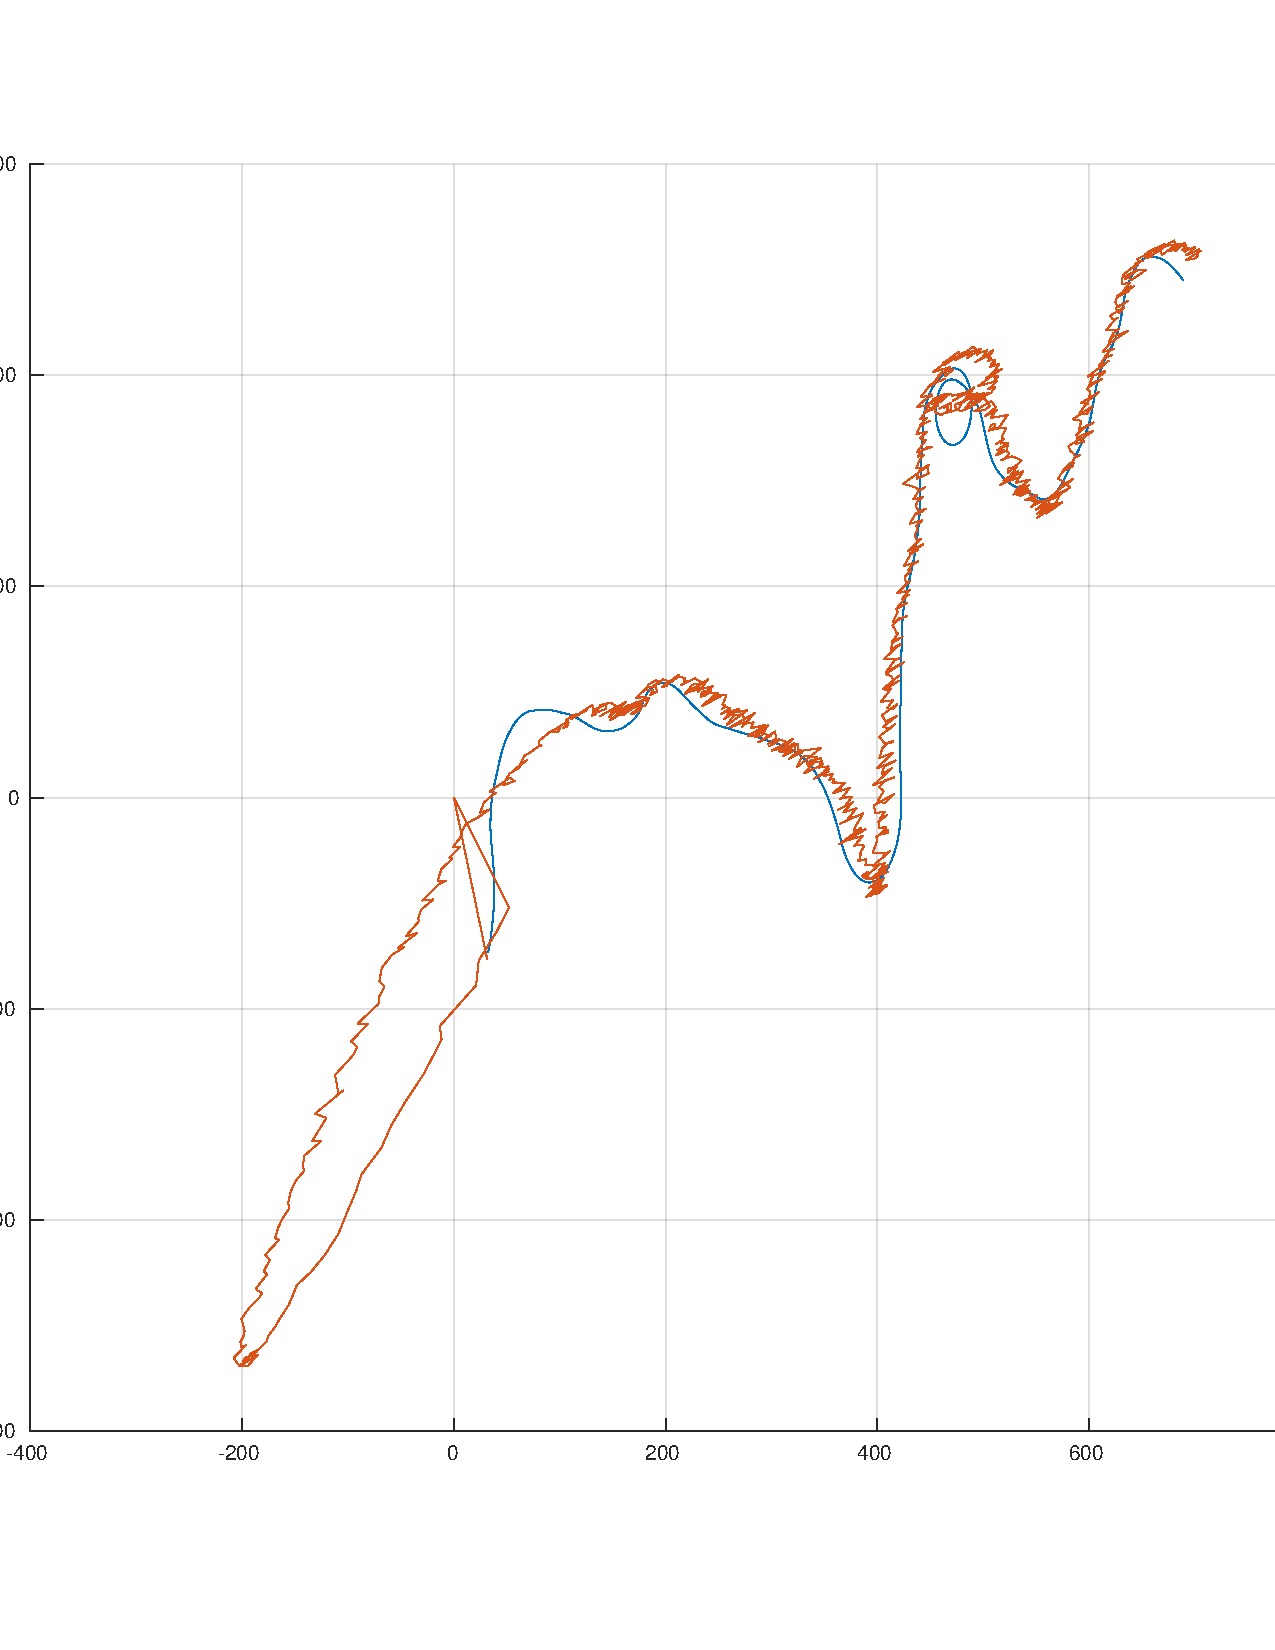
\includegraphics[width=\columnwidth]{ekf.pdf}
\caption{EKF performance. True state shown in blue, kalman filter estimate shown in red.}
\label{fig:ekf}
\end{figure}
As we see, the algorithm struggles with initializing, but then catches on. This can be caused by many things, but might in this case might simply be caused by a mistake in the formula, which is we it takes so long to get on the right track. We also notice the very "jagged" nature of the kalman filter estimate. This is caused by the kalman filter not giving us a realistic curve, but simply the best estimate given the data and the model at each timestep, hence the back-and-forth shape.


\end{document}

